\documentclass[a4paper,10pt]{article}

% PACKAGES
\usepackage[english, greek, francais]{babel}
\usepackage[utf8]{inputenc}
\usepackage[T1]{fontenc}
\usepackage{hyperref}
\usepackage{setspace}
\usepackage{latexsym}
\usepackage{graphicx}
\usepackage{csquotes}
\usepackage{bookman}
\usepackage{comment}
\usepackage{amsmath}
\usepackage{amssymb}
\usepackage{amsthm}
\usepackage{amscd}
\usepackage{color}
\usepackage{calc}
\usepackage{tikz}


% DIMENSIONS
\setlength{\voffset}{-3.75cm}
\setlength{\hoffset}{-2.6cm}
\setlength{\oddsidemargin}{2.75cm}
\setlength{\topmargin}{2in}
\setlength{\headheight}{0in}
\setlength{\headsep}{0in}
\setlength{\topskip}{0in}
\setlength{\parindent}{0cm}
\setlength{\parskip}{1ex plus0.4ex minus0.2ex}
\setlength{\textwidth}{16.25cm}
\setlength{\textheight}{21cm}
\renewcommand{\baselinestretch}{1.5}
\flushbottom
\setcounter{page}{1}
\setcounter{tocdepth}{2}


% COMMANDS
\newcommand{\guill}[1]{«~#1~»}
\newcommand{\eme}[0]{$^\text{e}$}
\newcommand*{\txtgreek}[1]{\foreignlanguage{greek}{#1}}


% ENVIRONMENTS


% THEOREMS
\theoremstyle{definition}
\newtheorem*{qq}{Question}
\newtheorem*{prob}{Problème}
\newtheorem*{nota}{Notation}
\newtheorem*{defi}{Définition}
\newtheorem*{ex}{Exemple}
\newtheorem*{rqu}{Remarque}
\newtheorem*{ledefi}{Défi}
\newtheorem*{ax}{Axiome}
\newtheorem*{exo}{Exercice}
\newtheorem*{rep}{$\longrightarrow$}
\theoremstyle{remark}
\theoremstyle{plain}


% DRAWINGS
\usetikzlibrary{positioning, chains, calc, arrows, decorations.pathreplacing, fit, calc}
\newcommand*\circled[1]{\tikz[baseline=(char.base)]{
            \node[shape=circle,draw,inner sep=2pt] (char) {#1};}}





\title{Sergej}
\begin{document}
\maketitle

\tableofcontents

\newpage

\section{Qu'est-ce que c'est?}

Sergej est un modèle neuronal numérique que nous appellerons "Cerveau" bien que ce n'en soit pas vraiment un.\\
Il suit des lois de connections qui modifient sa structure interne par le biais de rétroactions.

\section{Sergej et son environnement}

Sergej a besoin de signaux en entrée pour en restituer en sortie.
\begin{figure}
\centering
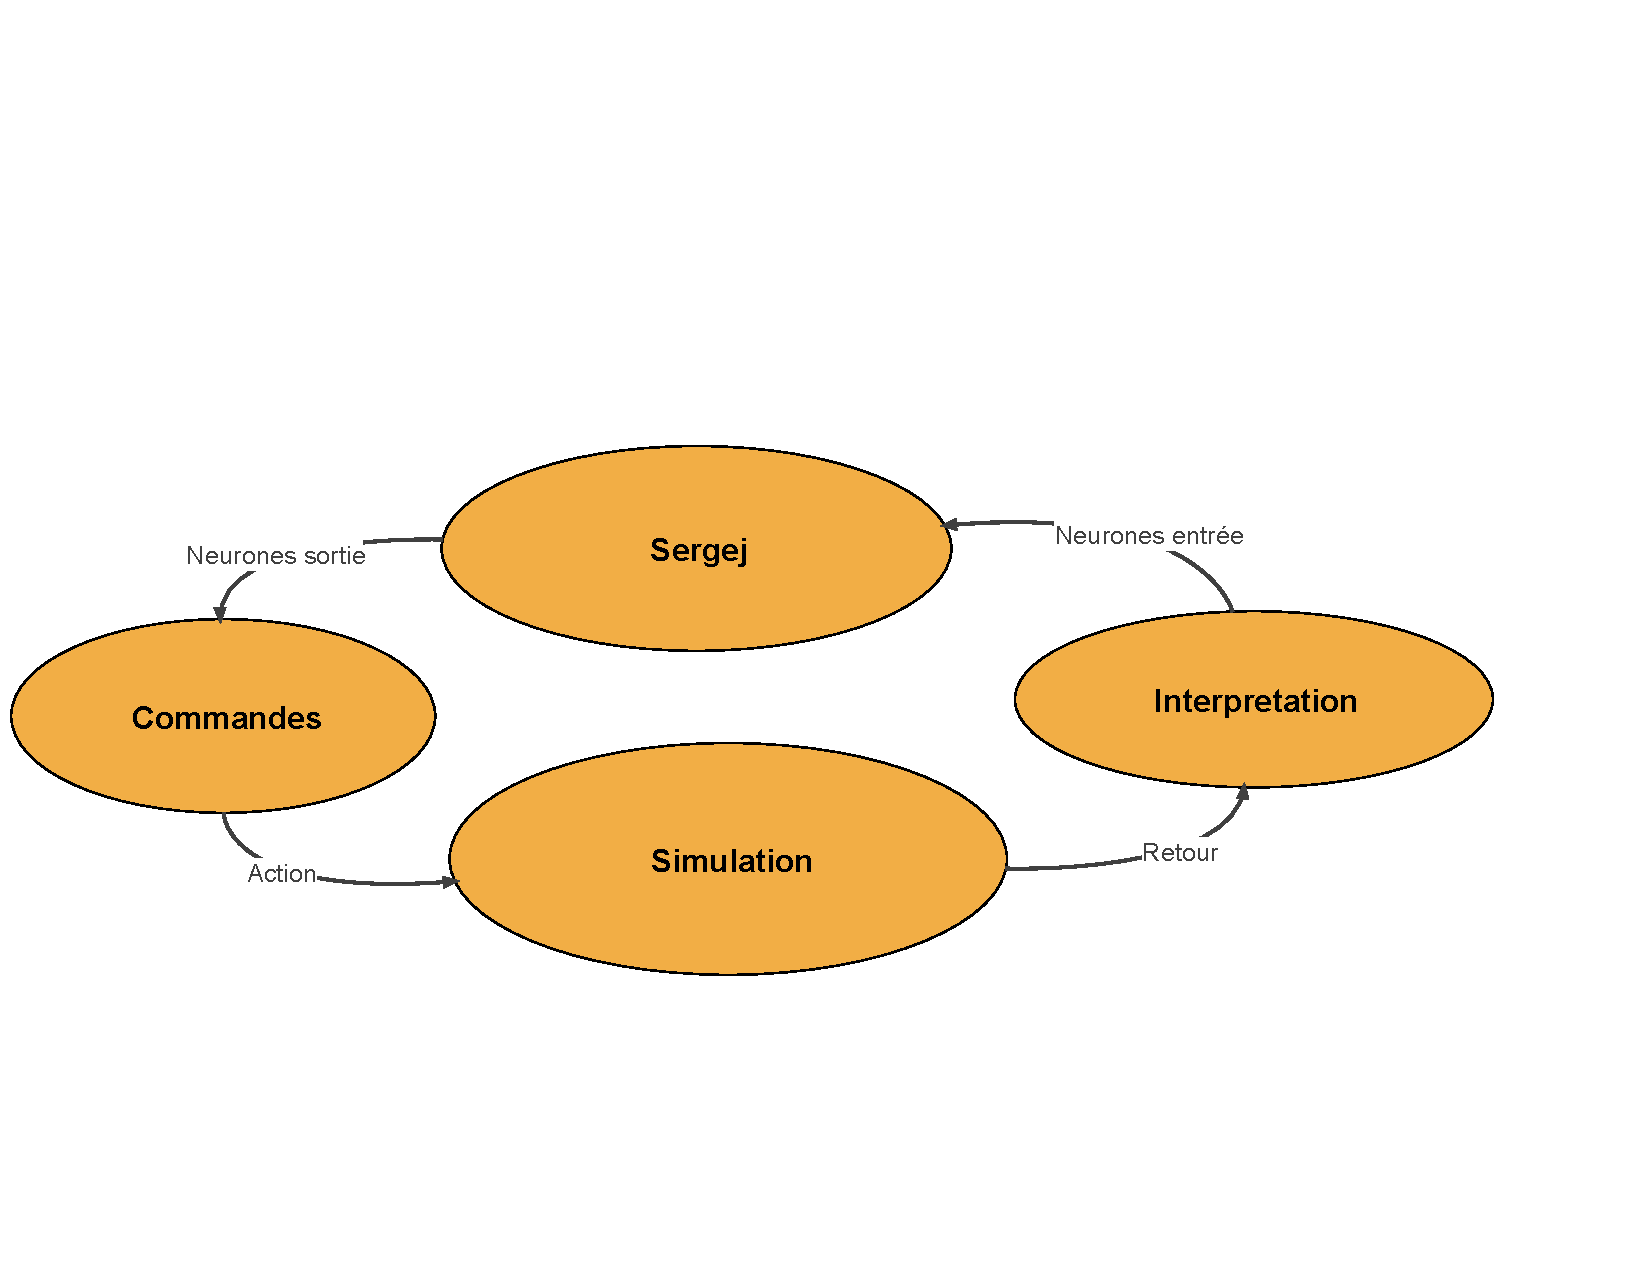
\includegraphics[scale=0.5]{System_commande_diagrame}
\caption{Sergej représenté dans son environnement}
\end{figure}

Le signal en entrée est transmit aux composantes internes de Sergej sommairement appelées neurones. Ces derniers, de même que Sergej reçoivent un signal en entrée pour en fournir un autre en sortie. Néanmoins à ce niveau un même neurone peut transmettre un signal à plusieurs congénères et de même pour ses entrées.

\begin{figure}
\centering
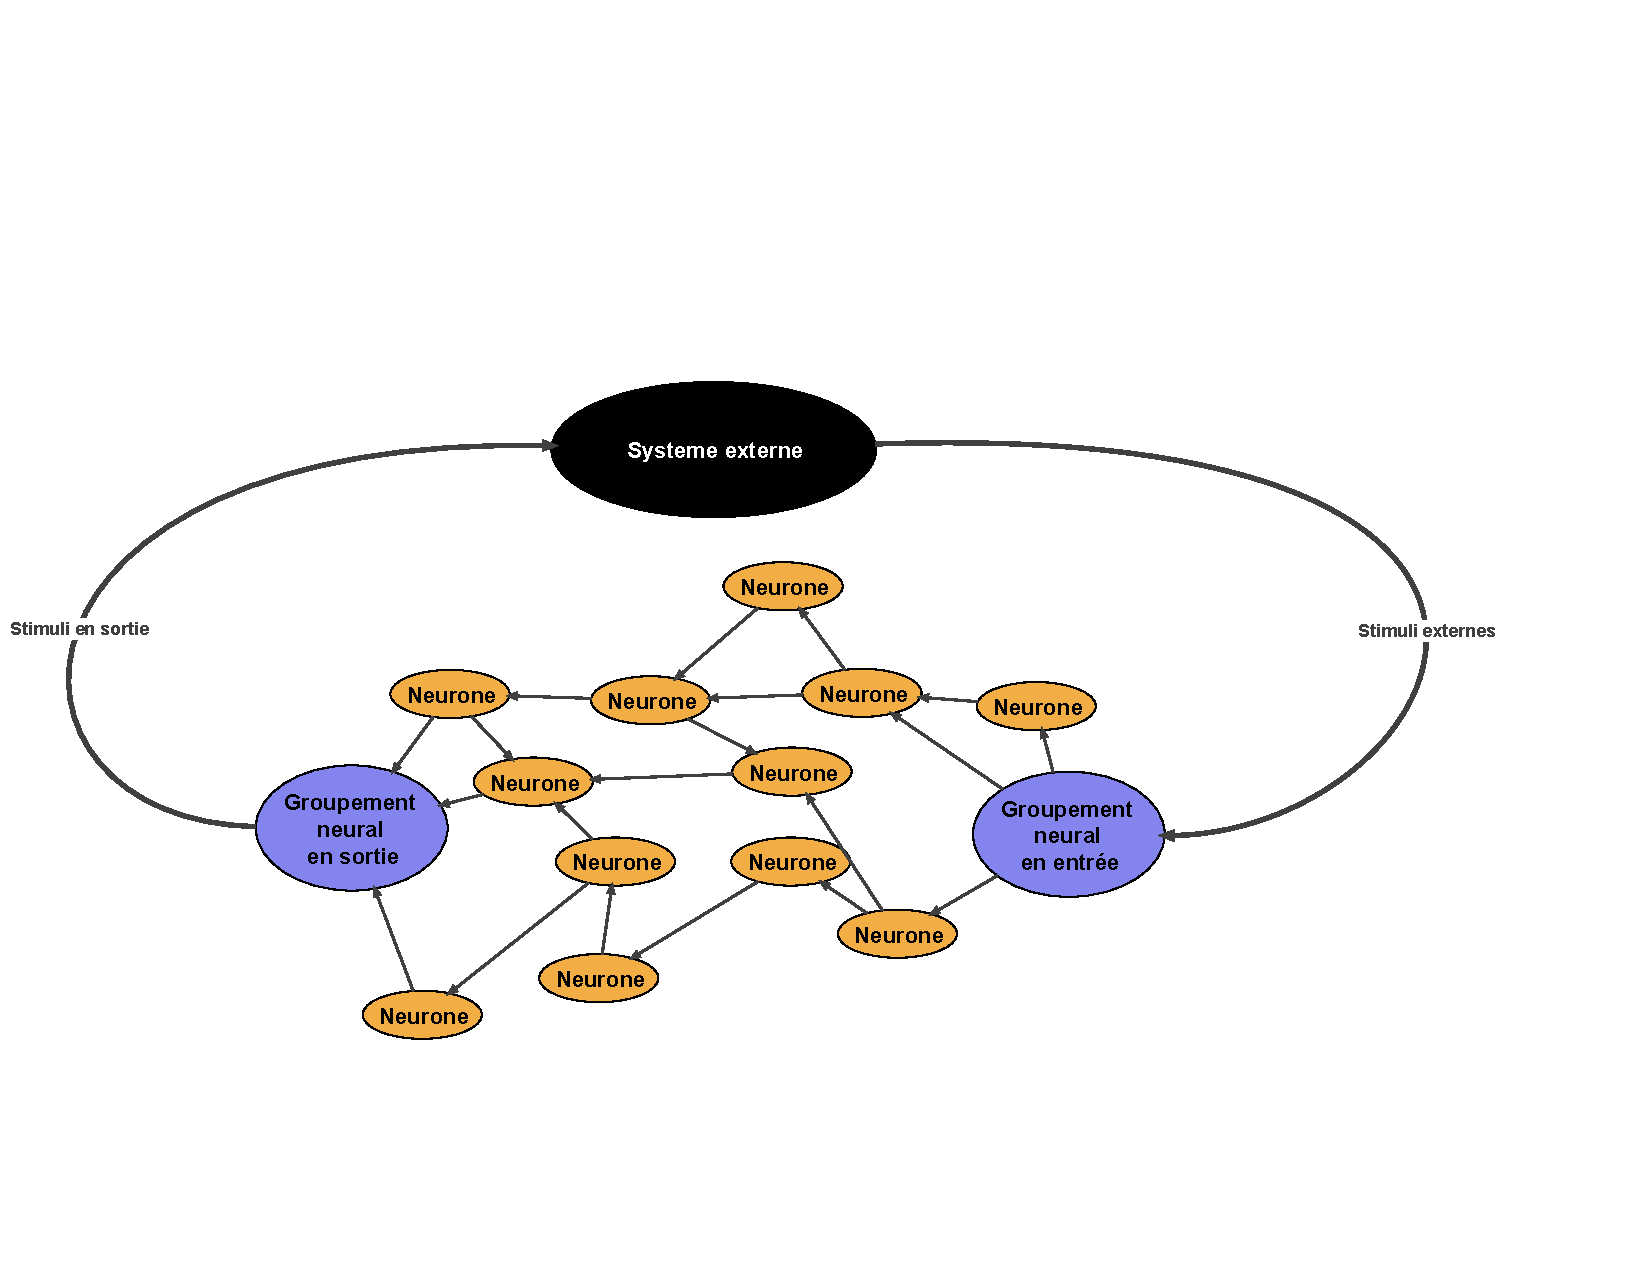
\includegraphics[scale=0.5]{Groupement_neural}
\caption{Schéma de l'architecture neurale interne}
\end{figure}

Des entités ayant la même structure mais à plus grande échelle (\guill{paquets} de neurones travaillant ensemble pour transformer un signal global d'entrée en signal global de sortie). Sergej ne serait-il pas qu'un seul grand neurone ? La question reste en suspens\dots

\section{Loi de génération et de positionnement}

Les groupements neuraux en entrée et en sortie doivent être générés \textit{avant} les autres afin de permettre à Sergej de communiquer avec son environnement. Par contre les neurones intermédiaires suivent des loi de génération et de positionnement.
\subsection{Loi de génération}
Exemples de lois de génération $G()$:
\begin{itemize}
\item Génération indépendante: Dans ce cas la génération de neurones dépend d'une loi externe au système dépendant, par exemple du temps. \\$G(t)=constante$, le nombre de neurones ajouté est toujours le même.\\
 $G(t)=\alpha\ln (t)$ le nombre de neurones ajoutés croit de moins en moins vite, etc...
\item Génération proportionnelle: Le nombre de neurones ajoutés dépend du nombre de neurones déjà présents.\\ $G(n) = K\left(\dfrac{1-\dfrac{n}{K}}{\alpha}\right)$ avec $\alpha\geq1$. Le nombre de neurones tend vers $K$.\\
\item Génération sur demande: Sergej dispose d'une commande générant des neurones.
\end{itemize}
\subsection{Loi de positionnement}

Une foi généré, un neurone doit être placé dans le réseau.


\section{Le \guill{bonheur}}

Pour que les actions du Cerveau puissent avoir un \emph{but}, même primitif, il doit pouvoir évaluer les conséquences de celle-ci. D'où la nécessité d'une mesure de \emph{bonheur} et, éventuellement, de \emph{malheur}.

\subsection{Bonheur universel}

Une première possibilité est de décrire le bonheur par le biais d'une variable globale, accessible immédiatement par tous les neurones. Chaque neurone, conservant alors l'historique de ses $n$ dernières actions, saura lesquelles ont eu des conséquences positives (augmentation du bonheur) ou négative (diminution). L'ampleur de ces conséquences correspond alors à la valeur absolue de la variation de bonheur.

\subsection{Bonheur neuronal}

Une autre possibilité consiste à attribuer la gestion la bonheur à un groupe spécifique de neurones. Ceux-ci auraient une forme générale de chaîne. Les neurones au début de la chaîne enverraient un signal correspondant à une variation de bonheur, qui serait transmis tout au long de la chaîne. Et chaque neurone du cerveau serait connecté en entrée à l'un des neurones de la chaîne du bonheur.

Dans ce cas, la chaîne doit être relativement courte par rapport au nombre total de neurones, pour que ceux-ci aient un retour sur leurs actions en temps raisonnable.

\subsection{Principe de plaisir et principe de réalité}

\paragraph{Principe de plaisir :} (tenter de) prédire si une action sera immédiatement suivie de bonheur. Pour cela, il suffit que les neurones possèdent un court historique (comprenant : leurs entrées, leur sortie, les actions éventuelles (augmenter/réduire le nombre de connexions), et la variation de bonheur consécutive), dont il tentent d'induire des lois de comportements.

\paragraph{Principe de réalité :} (tenter de) prédire sur le long terme quelles actions maximiseront le bonheur total, même si c'est au prix d'un malheur temporaire. Comment faire cela ? Par le biais d'une macro-structure enregistrant un historique sur le long terme ?


\end{document}